\chapter{Business Model Innovativi}

\section{Esca e amo}

Prevede la proposta di un prodotto (esca) ad un prezzo molto competitivo che
vincoli il cliente ad acquisti successivi (amo). Ovvero c'è un prodotto in sé e
un consumabile, che deve venire frequentemente riacquistato.

Questo non è un \textit{prodotto civetta}\footnote{Ovvero prodotti venduti da
grande catene di ridistribuzione che tramite volantinaggio fanno pubblicità,
invogliando a entrare nei propri negozi.}, perché si deve creare un vincolo che
obblighi a futuri acquisti ricorrenti.

\begin{example}[Prodotto civetta - Tesco]
Alla Tesco, i volantini e le promozioni sono studiati ad arte in quanto loro
pensano che ci siano 100-120 prodotti che sono dei \textbf{must have}, ovvero
prodotti per cui una persona è disposta ad uscire di casa per comprarli. Hanno
notato che sono presenti delle correlazioni tra questi prodotti e i
giorni della settimana (per esempio i pannolini con le birre il mercoledì, che
coincide con il giorno in cui le donne inglesi escono e lasciano i figli ai
padri) e sfruttano questa correlazione offrendo sconti mirati per invogliare
l'acquisto di determinati prodotti.
\end{example}

\noindent Esca e amo è presente spesso e volentieri nelle compagnie
telefoniche, che offrono telefoni con contratti. Questi telefoni sono dati a
prezzi molto scontati (se non gratis), ricavandoci tramite il contratto. L'unico
pericolo di questo genere di offerte sono la rescissione di quest'ultimo: è qui
che scatta il lock-in contrattuale, per evitare che il cliente salti da una
compagnia all'altra dopo che ha ricevuto il dispositivo.


\begin{figure}[t]
 \centering
 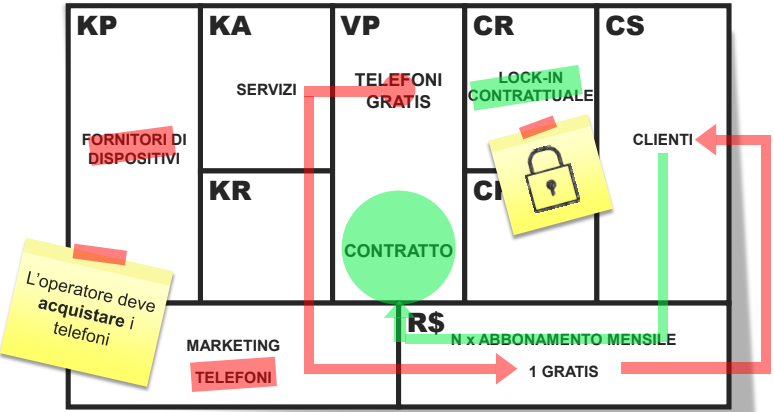
\includegraphics[scale=1.7]{bm_ex_tel}
 \caption[Business model per compagnia telefonica]{Esempio di un Business model
per una compagnia telefonica che offre telefoni a bassi prezzi tramite un
contratto.}
 \label{fig:bmi:ct}
\end{figure}

\begin{definition}[Comodity]
Sono quei prodotti considerati ormai di base per il nostro stile di vita che
non sono più differenziabili da un punto di vista della qualità. Prendere il
prodotto da un produttore o dall'altro non cambia molto\footnote{Le comodity
son molto pericolose da un punto di vista delle aziende perché l'unica cosa che
gli rimane in mano a loro a quel punto è fare leva sul prezzo.}.
\end{definition}

\noindent Altri casi di esca e amo sono relativi alla vendita di rasoi e
lamette. Ma mentre dal punto di vista della telefonia il telefono viene pagato
dalle compagnie telefoniche e rivenduto quasi a zero, in questo caso il prodotto
primario viene venduto sottocosto. Siccome non esistono vincoli contrattuali,
vengono ingegnati lock-in strutturali e impiegati brevetti per
impedire le rivendite di prodotti secondari da altri competitor. Bisogna
comunque prestare attenzione perché i brevetti non sono riconosciuti in tutti i
paesi e quindi tramite varie strade è sempre possibile far arrivare questi
prodotti secondari ai clienti.

In generale, questo modello di vendita si basa sul lock-in e sulla forza del
brand stesso: il prodotto primario che viene venduto sottoprezzo deve ispirare
fiducia ugualmente da parte del cliente. La gratificazione istantanea fa molta
leva in questo modello di vendita perché i prodotti secondari tenderanno ad
avere un costo maggiore della norma ma il prodotto primario, essendo di prezzo
molto competitivo, deve riuscire ad attrarre il cliente e ad spingerlo a
comprare.

\section{La coda lunga}

Questo termine è stato coniato da Chris Anderson per descrivere una
trasformazione che sta avvenendo nel mondo del business dei media, che sta
portando ad uno spostamento dalla vendita di un piccolo numero di ``hit'' in
grandi volumi, verso la vendita di grandi quantità di prodotti di nicchia,
ciascuno prodotto in piccole dosi.

\begin{example}[Case editrici]\label{ex:bi:ce}
Nell'esempio di una casa editrice, c'è tutto il costo fisso legato alla
stampa del libro più il prezzo da pagare all'autore e le spese di spedizione
alle librerie. La parte di selezione, come si può capire bene, diventa
fondamentale: scegliere i giusti autori determina la sopravvivenza della casa
editrice o meno. Ed è per questo motivo che a volte si trovano dei libri
pubblicati da personaggi famosi (come calciatori o veline) piuttosto che libri
d'autore che avrebbero una qualità maggiore ma un risalto più basso.
\end{example}

Con questo nuovo modello di vendita si è passati, riprendendo
l'Esempio~\ref{ex:bi:ce} dal vendere per pochi titoli famosi a molti titoli
meno famosi. Ovvero molte vendite, ciascuna delle quali poco frequenti,
producono ricavi aggregati pari o superiori a quelli generati dalla vendita di
poche hit.

Tutto ciò è derivato dall'avvento di internet: in particolare, ci sono stati
tre elementi scatenanti che hanno permesso la nascita di questo modello:
\begin{itemize}
 \item democratizzazione degli strumenti di produzione: milioni di appassionati
possono produrre film, registrare musica e scrivere software;
 \item democratizzazione della distribuzione: internet ha abbattuto i costi di
distribuzione di contenuti digitali, delle transazioni economiche e di
inventario e magazzino;
 \item crollo dei costi di ricerca per connettere domanda e offerta. La vera
sfida di vendere prodotti di nicchia è trovare potenziali acquirenti. Con
internet è diventato facile.
\end{itemize}

Alcuni esempi di aziende che hanno conseguito il seguente modello sono ad
esempio \url{lulu.com} come GettyImages, iStockPhoto e altri ancora.
L'importanza di questo modello sono i contenuti presenti nella piattaforma che
vende i prodotti. I contenuti si possono avere solo da autori, che fanno parte
però anche del mio \textit{customer segment}. Questo modello si focalizza
principalmente sui mercati di nicchia, ma può coesistere con il modello del
bestseller, unendo produttori che partono dal livello amatoriale per arrivare a
professionisti del settore. L'internet è l'elemento chiave: senza di esso
questo modello non può sussistere.

